% Aegis customer-service harness report. Every number is a macro from
% numbers.tex or a generated table (cs_harness/build_report.py). Do not type
% numbers into this file.
\documentclass[11pt]{article}

\usepackage[letterpaper,margin=1in]{geometry}
\usepackage[T1]{fontenc}
\usepackage[utf8]{inputenc}
\usepackage{lmodern}
\usepackage{microtype}
\usepackage{graphicx}
\usepackage{booktabs}
\usepackage{array}
\usepackage{xcolor}
\usepackage{caption}
\usepackage[colorlinks=true,allcolors=blue!50!black]{hyperref}

\captionsetup{font=small,labelfont=bf}
\setlength{\parskip}{0.45em}
\setlength{\parindent}{0pt}

% Generated by cs_harness/build_report.py -- do not edit.
\newcommand{\PlainPass}{26.2}
\newcommand{\PlainPassCI}{[15.0, 38.8]}
\newcommand{\PlainPassK}{0.0}
\newcommand{\PlainK}{4}
\newcommand{\PlainDb}{29.3}
\newcommand{\PlainCostConv}{0.0151}
\newcommand{\PlainCostSuccess}{0.057}
\newcommand{\PlainTrials}{4}
\newcommand{\PlainConvs}{80}
\newcommand{\PlainBlocked}{0}
\newcommand{\PlainFalseBlocks}{0}
\newcommand{\PlainRepaired}{0}
\newcommand{\CodePass}{43.8}
\newcommand{\CodePassCI}{[26.2, 61.3]}
\newcommand{\CodePassK}{25.0}
\newcommand{\CodeK}{4}
\newcommand{\CodeDb}{50.0}
\newcommand{\CodeCostConv}{0.0166}
\newcommand{\CodeCostSuccess}{0.038}
\newcommand{\CodeTrials}{4}
\newcommand{\CodeConvs}{80}
\newcommand{\CodeBlocked}{72}
\newcommand{\CodeFalseBlocks}{3}
\newcommand{\CodeRepaired}{1}
\newcommand{\LlmPass}{31.2}
\newcommand{\LlmPassCI}{[17.5, 46.2]}
\newcommand{\LlmPassK}{5.0}
\newcommand{\LlmK}{4}
\newcommand{\LlmDb}{32.5}
\newcommand{\LlmCostConv}{0.0215}
\newcommand{\LlmCostSuccess}{0.069}
\newcommand{\LlmTrials}{4}
\newcommand{\LlmConvs}{80}
\newcommand{\LlmBlocked}{227}
\newcommand{\LlmFalseBlocks}{17}
\newcommand{\LlmRepaired}{2}
\newcommand{\StrongPass}{47.5}
\newcommand{\StrongPassCI}{[32.5, 62.5]}
\newcommand{\StrongPassK}{20.0}
\newcommand{\StrongK}{4}
\newcommand{\StrongDb}{50.0}
\newcommand{\StrongCostConv}{0.0145}
\newcommand{\StrongCostSuccess}{0.031}
\newcommand{\StrongTrials}{4}
\newcommand{\StrongConvs}{80}
\newcommand{\StrongBlocked}{0}
\newcommand{\StrongFalseBlocks}{0}
\newcommand{\StrongRepaired}{0}
\newcommand{\PlainHumanPass}{27.5}
\newcommand{\PlainHumanPassCI}{[12.5, 42.5]}
\newcommand{\PlainHumanPassK}{10.0}
\newcommand{\PlainHumanK}{2}
\newcommand{\PlainHumanDb}{30.8}
\newcommand{\PlainHumanCostConv}{0.0106}
\newcommand{\PlainHumanCostSuccess}{0.038}
\newcommand{\PlainHumanTrials}{2}
\newcommand{\PlainHumanConvs}{40}
\newcommand{\PlainHumanBlocked}{0}
\newcommand{\PlainHumanFalseBlocks}{0}
\newcommand{\PlainHumanRepaired}{0}
\newcommand{\CodeHumanPass}{37.5}
\newcommand{\CodeHumanPassCI}{[20.0, 57.5]}
\newcommand{\CodeHumanPassK}{30.0}
\newcommand{\CodeHumanK}{2}
\newcommand{\CodeHumanDb}{42.1}
\newcommand{\CodeHumanCostConv}{0.0155}
\newcommand{\CodeHumanCostSuccess}{0.041}
\newcommand{\CodeHumanTrials}{2}
\newcommand{\CodeHumanConvs}{40}
\newcommand{\CodeHumanBlocked}{24}
\newcommand{\CodeHumanFalseBlocks}{3}
\newcommand{\CodeHumanRepaired}{4}
\newcommand{\BvADiff}{+17.5}
\newcommand{\BvACI}{[-1.2, +36.2]}
\newcommand{\BvAP}{0.088}
\newcommand{\BvABetter}{10}
\newcommand{\BvAWorse}{4}
\newcommand{\BvDDiff}{+12.5}
\newcommand{\BvDCI}{[-3.8, +27.5]}
\newcommand{\BvDP}{0.083}
\newcommand{\BvDBetter}{10}
\newcommand{\BvDWorse}{3}
\newcommand{\BvEDiff}{-3.8}
\newcommand{\BvECI}{[-27.5, +20.0]}
\newcommand{\BvEP}{0.777}
\newcommand{\BvEBetter}{7}
\newcommand{\BvEWorse}{9}
\newcommand{\DvADiff}{+5.0}
\newcommand{\DvACI}{[-10.0, +21.2]}
\newcommand{\DvAP}{0.696}
\newcommand{\DvABetter}{5}
\newcommand{\DvAWorse}{4}
\newcommand{\BhvAhDiff}{+10.0}
\newcommand{\BhvAhCI}{[-7.5, +27.5]}
\newcommand{\BhvAhP}{0.406}
\newcommand{\BhvAhBetter}{5}
\newcommand{\BhvAhWorse}{3}
\newcommand{\NTasks}{20}
\newcommand{\TestSpend}{6.45}
\newcommand{\DevSpend}{2.67}
\newcommand{\StudySpend}{9.13}
\newcommand{\DevPlainPassOne}{25.0}
\newcommand{\DevPlainPassTwo}{23.3}
\newcommand{\DevPlainFalseBlocks}{--}
\newcommand{\DevOnePassOne}{46.7}
\newcommand{\DevOnePassTwo}{40.0}
\newcommand{\DevOneFalseBlocks}{15}
\newcommand{\DevTwoPassOne}{58.3}
\newcommand{\DevTwoPassTwo}{50.0}
\newcommand{\DevTwoFalseBlocks}{8}

\newcommand{\AuthorName}{Varun Saran}
\newcommand{\RepoURL}{https://github.com/varunvsaran-wq/Aegis}

\title{\textbf{Checking a support agent's actions in code:}\\a harness that lifts a cheap model on airline customer service}
\author{\AuthorName}
\date{September 2026}

\begin{document}
\maketitle

\section*{Summary}

I built a harness that sits between a customer-service AI agent and the
airline database it works on. Before the agent can book, change, cancel or
compensate, the harness checks the action against the airline's written
policy, in code, using the real booking records. If the action breaks a rule,
it is not carried out; the agent is told exactly which rule and why, and gets
to try again.

I tested it on the airline tasks of $\tau^2$-bench, where an AI plays the
customer and a task only counts as solved if the database ends up exactly
right. On \NTasks{} held-out tasks, a cheap model (GPT-4o-mini) solved
\PlainPass\% of its attempts on its own and \CodePass\% with the harness. The
share of tasks it solved on every one of four tries went from \PlainPassK\% to
\CodePassK\%, and each solved task cost less (\$\CodeCostSuccess{} against
\$\PlainCostSuccess). With only \NTasks{} tasks
the improvement is large but not yet statistically certain (95\% interval
\BvACI{} points, $p = \BvAP$).

Two comparisons matter as much as the headline. The same harness with an AI
model doing the checking instead of code did much worse: it blocked
\LlmBlocked{} actions, \LlmFalseBlocks{} of them correct ones, and ended up
barely ahead of no harness at all. And the cheap model with the harness came
out level with a stronger model used on its own (\CodePass\% against
\StrongPass\%).

\section{Why this project}

This is the second version of Aegis. The first wrapped question answering on
HotpotQA and checked answers with another AI model. A controlled test showed
it mostly just declined to answer: its checker rejected correct answers about
as often as wrong ones, so every error it caught cost several right answers.

The research on this is fairly clear. A harness pays off when its checker is
exact, when a program can say for certain that something is wrong and exactly
what. Then the harness can make the model repair its work instead of giving
up. Company policy for a support agent is a good fit: most rules
(``basic economy flights cannot be changed'', ``a cancellation needs one of
these four conditions'') can be written as code against the booking database.

\section{What I built}

The agent is $\tau^2$-bench's own reference agent, with the same prompt and
the same model. The harness adds one step. Every tool call that would change
the database goes through a checker first:

\begin{itemize}
  \item \textbf{The checker} is the airline policy written as Python, from the
        policy document every agent is given. It reads the live database, never
        writes to it, and covers cancellation eligibility, flights already
        flown, basic-economy restrictions, route and trip-type rules on flight
        changes, checked-bag arithmetic, passenger counts, payment rules and
        compensation rules.
  \item \textbf{A blocked call} never reaches the database. The agent gets a
        tool result that names the problem, for example ``Reservation H9ZU1C is
        not eligible for cancellation: it was booked more than 24 hours ago, no
        flight was cancelled by the airline, the cabin is economy, and it has
        no travel insurance.''
  \item \textbf{Repair.} The agent can fix the call or tell the customer no.
        After two failed repairs it has to answer the customer in words.
  \item \textbf{One change at a time.} If the agent bundles several changes in
        one turn, only the first goes ahead, so later changes are judged
        against the database after the first has run.
\end{itemize}

Three rules depend on what the customer said, which code can only
approximate: whether they confirmed the change, whether a cancellation reason
is covered by insurance, and whether they asked for compensation. Those are
keyword rules and are marked as such in the code.

\section{How it was tested}

$\tau^2$-bench's airline domain has 50 tasks, split by its authors into 30 for
training and 20 for testing. I used the 30 training tasks to find and fix
problems in the checker, then froze it (the file hashes are in
\texttt{PROTOCOL.md}) and wrote down the test plan before running the 20 test
tasks once. The customer was played by GPT-4.1-mini in every run.

Each test task was run four times in each of four setups:

\begin{description}
  \item[A.] Plain agent, GPT-4o-mini.
  \item[B.] Harness with the code checker, GPT-4o-mini.
  \item[D.] Harness with an AI checker: the same model is shown the policy,
            the conversation, the proposed call and the same database records,
            and asked whether the call complies.
  \item[E.] Plain agent on a stronger model, GPT-4.1-mini.
\end{description}

A task attempt counts as solved only if $\tau^2$-bench's own scorer passes it:
the final database must match the reference and the agent must have told the
customer the required details. Comparisons are paired by task, with 95\%
bootstrap intervals over tasks and a Wilcoxon signed-rank test.

\section{Results}

\begin{figure}[h]
  \centering
  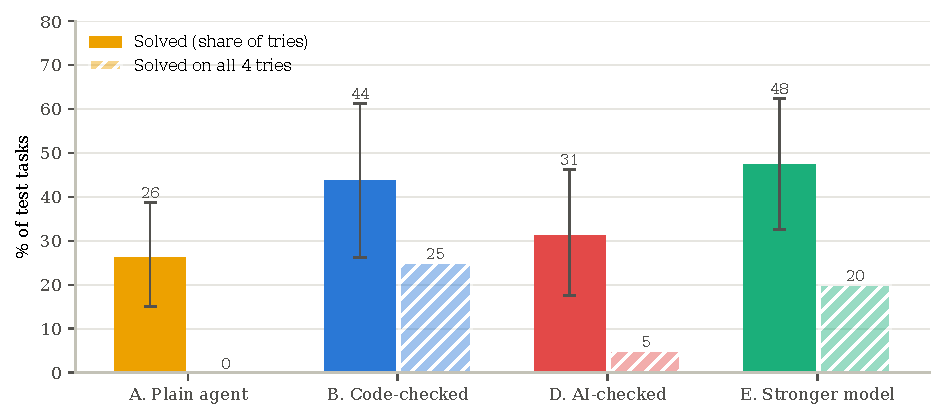
\includegraphics[width=\linewidth]{fig_main.pdf}
  \caption{Solid bars: share of attempts solved, with 95\% bootstrap intervals
    over the \NTasks{} test tasks. Hatched bars: share of tasks solved on all
    four tries.}
  \label{fig:main}
\end{figure}

\begin{table}[h]
  \centering\small
  \resizebox{\linewidth}{!}{\begin{tabular}{llrrrrrr}
\toprule
Arm & Agent & Solved (\%) & Solved every try & DB correct & \$/conv. & \$/solved & Blocks (false) \\
\midrule
A & Plain agent, gpt-4o-mini & 26.2 {\scriptsize[15.0, 38.8]} & 0.0\% & 29.3\% & 0.0151 & 0.057 & -- \\
B & Harness, code checker, gpt-4o-mini & 43.8 {\scriptsize[26.2, 61.3]} & 25.0\% & 50.0\% & 0.0166 & 0.038 & 72 (3) \\
D & Harness, AI checker, gpt-4o-mini & 31.2 {\scriptsize[17.5, 46.2]} & 5.0\% & 32.5\% & 0.0215 & 0.069 & 227 (17) \\
E & Plain stronger model, gpt-4.1-mini & 47.5 {\scriptsize[32.5, 62.5]} & 20.0\% & 50.0\% & 0.0145 & 0.031 & -- \\
\bottomrule
\end{tabular}
}
  \caption{Test results. Costs are in US dollars and include the agent, the
    simulated customer and, for D, the AI checker. ``False'' blocks are blocked
    calls identical to the reference answer's action.}
  \label{tab:main}
\end{table}

\paragraph{The code-checked harness.} It raised the solved share from
\PlainPass\% to \CodePass\%, doing better on \BvABetter{} tasks and worse on
\BvAWorse. The bigger change is in consistency (Figure~\ref{fig:passk}): the
plain agent never solved a test task on all four tries, while the harness did
so on \CodePassK\% of them. Most of its blocks stopped a real mistake; only
\CodeFalseBlocks{} of its \CodeBlocked{} blocks were on the correct action.

\begin{figure}[h]
  \centering
  \begin{minipage}{0.49\linewidth}\centering
    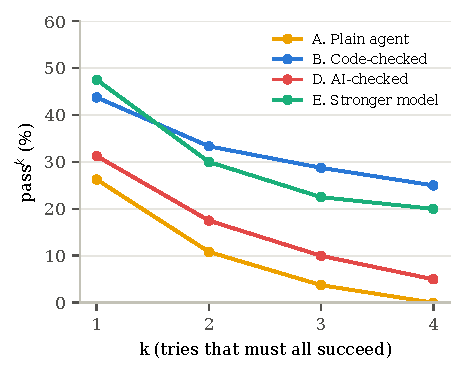
\includegraphics[width=\linewidth]{fig_passk.pdf}
  \end{minipage}\hfill
  \begin{minipage}{0.49\linewidth}\centering
    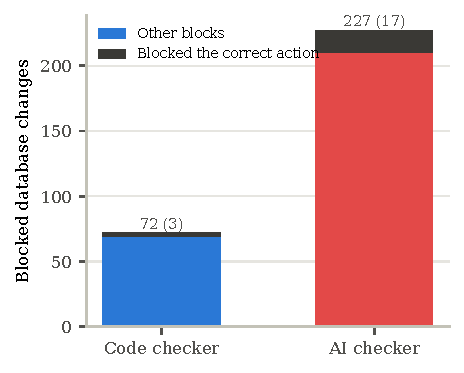
\includegraphics[width=\linewidth]{fig_checkers.pdf}
  \end{minipage}
  \caption{Left: pass$^k$, the share of tasks solved on all of $k$ tries.
    Right: database changes each checker blocked, and how many of those were
    the correct action.}
  \label{fig:passk}
\end{figure}

\paragraph{Code checker against AI checker.} This is the lesson from the
first Aegis, measured directly. Same model, same loop, same database records;
the only difference is who judges the call. The AI checker blocked
\LlmBlocked{} changes, three times as many as the code checker, and
\LlmFalseBlocks{} of them were the correct action. The agent spent its repairs
arguing with a checker that was often wrong, and the harness ended up
\DvADiff{} points over no checker at all ($p = \DvAP$). The code checker beat it
by \BvDDiff{} points ($p = \BvDP$).

\paragraph{Against a stronger model.} The cheap model with the harness solved
\CodePass\% of attempts; GPT-4.1-mini on its own solved \StrongPass\% (a
difference of \BvEDiff{} points, $p = \BvEP$, so no real difference). The
harness was more consistent (\CodePassK\% against \StrongPassK\% solved on
every try), and the stronger model was a little cheaper per solved task
(\$\StrongCostSuccess{} against \$\CodeCostSuccess). So the harness buys roughly
a model tier of reliability, not more.

\begin{table}[h]
  \centering\small
  \resizebox{\linewidth}{!}{\begin{tabular}{lrrrr}
\toprule
Comparison (paired by task) & Difference & 95\% CI & Wilcoxon $p$ & Tasks better / worse \\
\midrule
Code-checked vs plain & +17.5 pts & [-1.2, +36.2] & 0.088 & 10 / 4 \\
Code checker vs AI checker & +12.5 pts & [-3.8, +27.5] & 0.083 & 10 / 3 \\
Code-checked cheap model vs plain stronger model & -3.8 pts & [-27.5, +20.0] & 0.777 & 7 / 9 \\
AI-checked vs plain & +5.0 pts & [-10.0, +21.2] & 0.696 & 5 / 4 \\
Code-checked vs plain, human-like customer & +10.0 pts & [-7.5, +27.5] & 0.406 & 5 / 3 \\
\bottomrule
\end{tabular}
}
  \caption{Paired comparisons over the \NTasks{} test tasks. The last row used
    two tries per task instead of four.}
  \label{tab:comparisons}
\end{table}

\paragraph{Human-like customers.} I also ran the plain agent and the harness
against a more realistic simulated customer. It writes short, casual messages,
gives details only when asked and gets impatient, but keeps every goal and
every ID exactly as in the task. The harness still helped (\CodeHumanPass\%
against \PlainHumanPass\%), but with two tries per task that difference is not
reliable ($p = \BhvAhP$).

\paragraph{What the checker caught.} Table~\ref{tab:examples} shows real test
conversations, picked automatically. In the first three the plain agent failed
the task on every try and the harness solved it; in each, the harness stopped
a cancellation the policy does not allow. The last row is a task where the
harness did worse than the plain agent.

\begin{table}[!t]
  \centering\footnotesize
  \begin{tabular}{>{\raggedright\arraybackslash}p{0.05\linewidth}>{\raggedright\arraybackslash}p{0.24\linewidth}>{\raggedright\arraybackslash}p{0.21\linewidth}>{\raggedright\arraybackslash}p{0.32\linewidth}>{\raggedright\arraybackslash}p{0.07\linewidth}}
\toprule
Task & Customer's opening message & Blocked call & What the checker told the agent & Result \\
\midrule
24 & Hi! I need to remove a passenger named Ethan from my reservation with the code H9ZU1C. Can you help me with that? & \texttt{cancel\_reservation} & Reservation H9ZU1C is not eligible for cancellation: it was booked 2024-05-01 04:50 (more than 24 hours ago), no flight was cancelled by the airline, the cabin is economy, and it has no travel insurance. Deny the request. & Solved \\
44 & Hi, I need to review all my upcoming flight reservations. I want to cancel any flights that are longer than 4 hours. Fo... & \texttt{cancel\_reservation} & Reservation S61CZX can only be cancelled under its travel insurance, which covers health or weather reasons. Confirm the customer's reason; a change of plans is not covered, so the request must be denied. & Solved \\
45 & Hi, this is Sophia Taylor. I need to cancel my flight immediately due to a family emergency. My reservation number is P... & \texttt{cancel\_reservation} & Reservation PEP4E0 is not eligible for cancellation: it was booked 2024-05-05 05:10 (more than 24 hours ago), no flight was cancelled by the airline, the cabin is basic\_economy, and it has no travel insurance. Deny the request. & Solved \\
\midrule
8 & Hi! I'd like to book a one-way flight from ORD to PHL on May 26. I want to book the exact same flight I took recently o... & \texttt{book\_reservation} & Payment method certificate\_5094406 is not in the user's profile; only saved methods can be used. & Failed \\
\bottomrule
\end{tabular}

  \caption{Real test conversations. Top: tasks the plain agent never solved
    and the harness did, with the first block in that conversation. Bottom: a
    task where the harness did worse than the plain agent.}
  \label{tab:examples}
\end{table}

\section{What changed during development}

The first version of the checker was too strict in ways the policy is not. It
blocked any turn with more than one tool call, and it required a database
lookup of the customer where the policy only asks for their user id. In a first
trial on three training tasks most of its blocks came from those two rules, so
I relaxed both to match the policy text.

Checking every block against the reference answers on the training tasks
showed where the rest of the false blocks came from. The exact rules (routes,
bag arithmetic, flown segments) never blocked a correct action. The false
blocks came from the keyword rule for confirmation, which missed direct
instructions such as ``Just cancel both reservations'', and from a timing bug:
when the agent upgraded a booking and cancelled it in the same turn, the
checker judged the cancellation against the booking before the upgrade. I
fixed both and stopped there.

\begin{table}[h]
  \centering\small
  \begin{tabular}{lrrr}
\toprule
Development set (30 tasks $\times$ 2 tries) & Solved (\%) & Solved both tries (\%) & False blocks \\
\midrule
Plain agent & 25.0 & 23.3 & -- \\
Harness, first version & 46.7 & 40.0 & 15 \\
Harness, final version & 58.3 & 50.0 & 8 \\
\bottomrule
\end{tabular}

  \caption{Training tasks only. False blocks are blocked changes identical to
    the reference action.}
  \label{tab:dev}
\end{table}

I left one known disagreement in place. One training task's reference answer
cancels an insured economy booking because the customer's plans changed. The
policy says insurance covers only health and weather, so the checker blocks
it. Following the written policy costs points on that task, and I preferred
that to tuning the checker toward the benchmark's answers.

\section{Limitations}

\paragraph{Twenty tasks.} The test split is small. The harness's gain over
the plain agent is large but its 95\% interval (\BvACI{} points) still reaches
just below zero. A larger domain, such as $\tau^2$-bench retail with more than
100 tasks, would settle it.

\paragraph{One domain and a simulated customer.} All results are on airline
tasks, with another AI playing the customer. Simulated customers make their
own mistakes, and a real deployment would face messier requests.

\paragraph{Keyword rules.} Three rules read the customer's words with keyword
patterns. On the training tasks they caused most of the false blocks that
remained after the fixes; I did not break down the test-set false blocks by
rule.

\paragraph{What the checker can't fix.} In the training runs some failures had
nothing to do with policy: the agent made the right change but never told the
customer a required figure, such as a price difference. A checker on database
changes can't catch that.

\section{Cost}

Development cost \$\DevSpend{} and the test runs \$\TestSpend{}, \$\StudySpend{}
in total, including the simulated customers and the AI checker.

\section{Reproducing}

The code is in the \texttt{cs\_harness/} folder of

\url{\RepoURL}

Its \texttt{README.md} and \texttt{PROTOCOL.md} list the exact commands. With an
OpenRouter key in \texttt{.env}, one test arm is:

\begin{verbatim}
cd third_party/tau2-bench
.venv/Scripts/python.exe ../../cs_harness/run.py run \
  --domain airline --task-split-name test \
  --agent guarded_code_agent --num-trials 4 \
  --agent-llm openrouter/openai/gpt-4o-mini \
  --user-llm openrouter/openai/gpt-4.1-mini \
  --save-to test_B_code_4omini
\end{verbatim}

\texttt{cs\_harness/analyze.py} computes the statistics and
\texttt{cs\_harness/build\_report.py} regenerates every number, table and figure
in this document.

\end{document}
